% !TEX TS-program = xelatexmk
% !TEX encoding = UTF-8 Unicode
%
% Compile this document using xelatex
\documentclass{report}

% Enable links in the PDF, but make them colored black
\usepackage[%
  colorlinks,
  linkcolor=black,
  anchorcolor=black,
  citecolor=black,
  filecolor=black,
  menucolor=black,
  runcolor=black,
  urlcolor=black,
  bookmarksopen=true,
  pdfpagelabels
]{hyperref}

% Make dates like this: 15 January 2013
\usepackage[english,cleanlook]{isodate}

% Make citations look like this: (Jones, 1979)
\usepackage{natbib}
\setcitestyle{round,semicolon}

% Make xelatex use latex mappings (such as --- for em-dash)
\usepackage{fontspec}
\defaultfontfeatures{Mapping=tex-text}

% Use Tikz to draw
\usepackage{tikz}
\usetikzlibrary{arrows,shapes,snakes,automata,backgrounds,petri}


\title{Ducttape Technical Report}
\author{Lane Schwartz \and Jonathan Clark}

\begin{document}
\maketitle
\tableofcontents

\chapter{Motivation}

\citep{pedersen08}


\citep{deelmanetal09}

\citep{schwartz10} using GNU Make \citep{gnumake}

LoonyBin \citep{clarklavie10,clarketal10}

EMS \citep{koehn10ems}
  
Ducttape \citep{ducttape}

\chapter{The ducttape hyperworkflow language}

\chapter{HyperDAG theory}

\section{DAG --- directed acyclic graphs}

\section{HyperDAG --- directed acyclic hypergraphs}

\section{MetaHyperDAG --- directed acyclic hypergraphs with epsilon vertices}

\section{PhantomMetaHyperDAG --- directed acyclic hypergraphs with epsilon and phantom vertices }



\chapter{Building a workflow}

\section{Parsing a tape file}

Parsing is initiated by the ducttape main method through a call to \texttt{ducttape.syntax.\-GrammarParser.readWorkflow()}.
%
This causes the ducttape text file(s) to be parsed, ultimately resulting in an abstract syntax tree (AST).
%
\texttt{GrammarParser.readWorkflow()} calls \texttt{GrammarParser.parseAll()} to perform the actual parsing.
%
The result of is a sequence of objects directly representing the elements in the tape file;
the type of each element is \texttt{ducttape.syntax.ASTType}.

This list of elements is used to construct a \texttt{ducttape.syntax.WorkflowDefinition} object.
%
The ducttape main method similarly reads and parses any config files specified by the user, resulting in other \texttt{WorkflowDefinition} object(s).
%
All \texttt{WorkflowDefinition} objects are concatenated together into a single object --- \texttt{val wd: WorkflowDefinition}.
%
This object is error-checked by \texttt{StaticChecker} and by \texttt{WorkflowChecker}.

Finally, the \texttt{WorkflowDefinition} is used to construct a \texttt{ducttape.workflow.\-builder.WorkflowBuilder}.
%
The \texttt{WorkflowBuilder.build()} method is responsible for converting the AST into a \texttt{HyperWorkflow}.

%\begin{enumerate}
%\item 
%\end{enumerate} 


\section{Branch points and branches}
\label{sec:branchpoints_branches}
The \texttt{WorkflowBuilder.build()} method begins by traversing the abstract syntax tree represented by the \texttt{WorkflowDefinition}, looking for branch points and branches.
%
\texttt{WorkflowBuilder} has member variables \texttt{branchPointFactory} and \texttt{branchFactory} that maintain maps from branch point names to \texttt{BranchPoint} objects and branch names to \texttt{Branch} objects, respectively.
%
This traversal is performed by the inner method \texttt{findBranchPoints}.
%
After \texttt{findBranchPoints} is run, \texttt{branchPointFactory} and \texttt{branchFactory} have been populated with all branch points and branches in the workflow.

%
%\begin{enumerate}
%
%\item Traverse the AST to identify all branch points used in the workflow 
%      (see \texttt{findBranchPoints()} in \texttt{WorkflowBuilder.build()}; also 
%       see \texttt{BranchPoint} and \texttt{BranchPointFactory})
%
%\item For each branch point, identify all branch names associated with that branch point 
%      (see \texttt{Branch} and \texttt{BranchFactory}, especially \texttt{BranchFactory.getAll()})
%
%\end{enumerate}


\section{Building task templates}
\label{sec:buildTaskTemplates}

After identifying branch points and branches (\S\ref{sec:branchpoints_branches}), the \texttt{WorkflowBuilder.build()} method next constructs a \texttt{TaskTemplateBuilder} object from the \texttt{WorkflowDefinition}, the \texttt{BranchPointFactory}, and the \texttt{BranchFactory}.
%


\subsection{Find tasks}

After creating a \texttt{TaskTemplateBuilder} (\S\ref{sec:buildTaskTemplates}), the \texttt{WorkflowBuilder.build()} method calls \texttt{TaskTemplateBuilder.findTasks()}.
%
The \texttt{TaskTemplateBuilder.findTasks()} method is responsible for identifying temporal and structural dependencies among tasks and store those dependencies as an edge map; this method is also responsible for pre-resolving any non-temporal dependencies such as parameters.

%See \texttt{TaskTemplateBuilder.findTasks()}, called from \texttt{WorkflowBuilder.build()}

The \texttt{TaskTemplateBuilder.findTasks()} method performs the following actions:

\begin{enumerate}

\item The \texttt{findTasks()} method first gather a list of all task definitions present in the \texttt{WorkflowDefinition}. This includes regular task definitions as well as task definitions constructed by function calls.

\item By iterating over this list of task definitions, the \texttt{findTasks()} method next constructs a map where 
      the keys are globally unique task names and 
      the values are task definitions --- \texttt{taskMap: Map[Namespace,TaskDef]}.

\item For each task, iterate over all input specifications and parameter specifications for that task
      (see \texttt{TaskTemplateBuilder.findTasks()})

\item This step is extremely complicated and involves several mutually recursive functions.
      For each input specification and parameter specification in a task, 
      collect the set of possible values that each input and parameter can take. 
      This set of possible values will be recorded as a \texttt{BranchPointTree}.
      See \texttt{TaskTemplateBuilder.resolveBranchPoint()}, called from \texttt{TaskTemplateBuilder.findTasks()}.
      
\item BranchGraft elements are currently handled within \texttt{TaskTemplateBuilder.resolveNonBranchVar()}

\end{enumerate}

This results in a \texttt{TaskTemplateBuilder.parents} map, with tasks as keys, and values as follows:

\texttt{TaskTemplate} -> \texttt{BranchPointTreeGrafts}, which maps a \texttt{BranchPointTree} to a \texttt{Seq[Branch]} set of grafts
    
    \quad \texttt{BranchPointTree}, which contains an \texttt{ArrayBuffer[BranchTree]}, listing this BP's corresponding branches
    
    \quad A \texttt{Baseline} BP: all tasks have a \texttt{Baseline} BP, with a \texttt{baseline} branch. If the task has no BPs, \texttt{Baseline} has no children.
        
        \quad \quad \texttt{BranchTree}, which contains an \texttt{ArrayBuffer[TerminalData]} and an \texttt{ArrayBuffer[BranchPointTreeGrafts]}(children)
        
        \quad \quad A \texttt{Baseline.baseline} branch, containing \texttt{TerminalData} and an \texttt{ArrayBuffer[BranchPointTreeGrafts]} of children
            
            \quad \quad \quad \texttt{TerminalData}: only leaves have \texttt{TerminalData}, one for each dependency
                
                \quad \quad \quad \quad \texttt{task}: the (highest) task these specs depend on; type: \texttt{Option[TaskDef]}
                
                \quad \quad \quad \quad \texttt{grafts}: any grafts that were applied to these specs; type: \texttt{List()}
                
                \quad \quad \quad \quad \texttt{isParam}: true if literal, false if temporal; type: \texttt{Boolean}
                
                \quad \quad \quad \quad \texttt{specs}: used to resolve literals; type: \texttt{ArrayBuffer[SpecPair]}
                    
                    \quad \quad \quad \quad \quad \texttt{origSpec}: the variable name; type: \texttt{Spec}
                    
                    \quad \quad \quad \quad \quad \texttt{srcTask}: the source task of the value; type: \texttt{Option[TaskDef]}
                    
                    \quad \quad \quad \quad \quad \texttt{srcSpec}: the value assigned to the variable; type: \texttt{SpecT}
            
            \quad \quad \quad \texttt{Children}, an \texttt{ArrayBuffer[BranchPointTreeGrafts]} in which nested BPs appear


\begin{description}
\item[abc] ntshaonsetu snthsaonetus ntaoheus sanothes
\item[def] thsatnohusnth snthasuntaeh
\item[ghi] \ \\
      \begin{description}
          \item[baz] nested level 2
          \item[] thsnth sthnsnth
          \item[] tsnhaoeustnh
      \end{description}
\end{description}



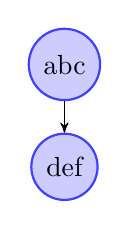
\begin{tikzpicture}[node distance=1.3cm,>=stealth',bend angle=45,auto]

  \tikzstyle{branch}=[circle,thick,draw=blue!75,fill=blue!20,minimum size=6mm]
  \tikzstyle{branchpoint}=[place,draw=red!75,fill=red!20]
  \tikzstyle{task}=[rectangle,thick,draw=black!75,fill=black!20,minimum size=4mm]

  \node [branch] (b1)                                    {abc};
  \node [branch] (b2)   [below of=b1]                    {def};

  \draw [->] (b1) -- (b2);

\end{tikzpicture}


\section{Temporal and structural dependencies}

\section{Constructing a packed hyperDAG}

See \texttt{WorkflowBuilder.build()}

\begin{enumerate}

\item For each task template, create a vertex. Store these vertices in a map, where the keys are globally-unique task names.

\item Build a sequence of Hyperedges, consisting of both nestedBranchEdges and terminalEdges, in which nested branch points and
      literals are assigned phantom edges and all other vertices are assigned normal edges.

\item Call \texttt{traverse} on each phantom vertex, recursively adding meta edges as appropriate. Meta edges map Branches to 
      BranchPoints one-to-one, as opposed to Hyperedges, in which multiple Branches can share the same sink.

\end{enumerate}


\bibliographystyle{plainnat}
\bibliography{report}

\end{document}
